\documentclass{beamer}
\mode<presentation>
\usepackage{amssymb,textcomp}
%\usepackage{beamerthemesplit}
\usepackage{beamerthemeJuanLesPins}
\usepackage{verbatim}
\usepackage{algorithm2e}
\usefonttheme{serif}
\title{Unidad I: Teor\'ia de Aproximaci\'on.}
\author{Jos\'e Luis Ram\'irez B.}
\date{\today}

\begin{document}

\frame{\titlepage}

\frame{\tableofcontents}

\section{Introducci\'on}
\begin{frame}[fragile]
  \frametitle{Motivaci\'on.} 
  \begin{itemize}
    \item<1-> La gran mayor\'ia de los modelos matem\'aticos que describen procesos f\'isicos no pueden resolverse anal\'iticamente.
    \item<2-> En una situaci\'on pr\'actica, un problema matem\'atico deriva de un fen\'omeno f\'isico sobre el cual se han hecho algunas suposiciones para simplificarlo y poderlo representar matem\'aticamente.
    \item<3-> Una vez formulado el problema, deben dise\~narse m\'etodos num\'ericos para resolver el problema. La selecci\'on o construcci\'on de los algoritmos apropiados cae propiamente dentro del terreno del An\'alisis Num\'erico.
  \end{itemize}    
\end{frame}
%%%%%
\section{Teor\'ia de Errores y Aproximaci\'on.}
\begin{frame}[fragile]
  \frametitle{Teor\'ia de Errores y Aproximaci\'on.}
  El an\'alisis num\'erico proporciona m\'etodos computacionales para el estudio y soluci\'on de problemas matem\'aticos. Debido a que muchos c\'alculos son realizados en computadores digitales, es conveniente la discusi\'on para la implementaci\'on de los m\'etodos num\'ericos como programas de computador..
\end{frame}
%%%%%
\begin{frame}[fragile]
  \frametitle{Teor\'ia de Errores y Aproximaci\'on.}
\begin{itemize}
  \item La aparici\'on de computadores ha hecho posible la soluci\'on de problemas, que por su tama\~no antes eran
  excluidos.
  \item<2-> Desafortunadamente los resultados son afectados por el uso de la Aritm\'etica de Precisi\'on Finita.
  \item<3-> Esperamos tener siempre expresiones verdaderas como $2+2=4$, $3^2=9$, $(\sqrt{5})^2 = 5$, pero en la aritm\'etica de precisi\'on finita $\sqrt{5}$ no tiene un solo n\'umero fijo y finito, que lo representa.
  \item<4-> En el computador se le da un valor aproximado cuyo cuadrado no es exactamente 5, aunque con toda probabilidad estar\'a lo bastante cerca a \'el para que
  sea aceptable.
\end{itemize}  
\end{frame}
%%%%%
\begin{frame}
  \frametitle{Teor\'ia de Errores y Aproximaci\'on.}
  Un m\'etodo num\'erico es un procedimiento mediante el cual se obtiene, de manera aproximada, la soluci\'on de ciertos problemas. Los resultados num\'ericos est\'an influenciados por muchos tipos de errores, los cuales pueden ser catalogados a  grandes rasgos en tres tipos b\'asicos:
  
  \begin{itemize}
   \item<2-> \textbf{Errores inherentes} que existen en los valores de los datos de entrada, ya sea causados por incertidumbre o por la naturaleza necesariamente aproximada de la representaci\'on.
    \item<3-> \textbf{Errores de discretizaci\'on} (llamados tambi\'en de truncamiento) que surgen al reemplazar procesos l\'imites por su resultado antes de alcanzar tal l\'imite.
    \item<4-> \textbf{Errores de redondeo} que se originan al utilizar una aritm\'etica que involucra n\'umeros con un n\'umero finito de d\'igitos.
  \end{itemize}
\end{frame}
%%%%%%
\frame
{
  \frametitle{Errores Absolutos y Relativos.}


  Sea $x$ el valor exacto de un n\'umero real y $\tilde{x}$ el valor aproximado. Contemplando todos los posibles errores, la relaci\'on entre el resultado exacto y el aproximado es:
$$
x = \tilde{x}+E
$$

\uncover<2->{
Se define el error absoluto y se denota $E_a$ como la diferencia $x-\tilde{x}$, y se expresa siempre en valor absoluto.
\begin{block}{}
 $$
 E_a = |x-\tilde{x}|
 $$
\end{block}}
}
%%%%
\frame{
\frametitle{Forward and Backward Error}
\begin{itemize}
   \item Sea $x$ un n\'umero real y $f:\mathbb{R}\to\mathbb{R}$ una funci\'on. Si $\tilde{y}$ es un 
n\'umero real que es una aproximaci\'on a $y=f(x)$, entonces el error hacia adelante (Forward) en 
$\tilde{y}$ es la diferencia $\Delta y=\tilde{y}-y$.
\item<2-> Sea $x\in \mathbb{R}$ y $f:\mathbb{R}\to\mathbb{R}$ una funci\'on. Sup\'ongase que 
$\tilde{y}$ es una aproximaci\'on a $y=f(x)$ y $\tilde{y}$ est\'a en el rango de $f$, es decir, 
$\tilde{y}=f(\tilde{x})$ para alg\'un $\tilde{x}$, entonces la cantidad $\Delta x=\tilde{x}-x$ es 
el error hacia atr\'as (Backward) en $\tilde{y}$.
\end{itemize}
}
%%%
\frame{
\frametitle{Forward and Backward Error}
\underline{Ejemplo:}

Sup\'ongase que se desea calcular $y=\sqrt{2}$ y se obtiene $\tilde{y}=1.4$, entonces:
\begin{itemize}
   \item<2-> Forward Error: $|\Delta y|=|\tilde y - y|=|1.4-1.4142\ldots|\approx 0.0142\ldots$
   \item<3-> Backward Error: N\'otese que $\sqrt{1.96}=1.4$, entonces  $|\Delta 
x|=|\tilde{x}-x|=|1.96-2|=0.04$
\end{itemize}
}
%%%%
\frame
{\frametitle{Errores Absolutos y Relativos.}

Una debilidad de esta definici\'on es que la magnitud del error verdadero depende de la escala. 
\begin{itemize}
 \item<2-> Por ejemplo podemos medir una barra en cent\'imetros o en metros. Si la longitud exacta de la barra es $1m$ 
y por la medici\'on se obtiene $99cm$, 
\begin{enumerate}
 \item<3-> $E_a = 100 - 99 = 1$, si usamos cent\'imetros.
 \item<4-> $E_a = 1.00 - 0.99 = 0.01$, si usamos metros.
\end{enumerate}
\end{itemize}

\uncover<5->{Esta es la raz\'on por la que se define el error relativo.}
}
%%%%
\frame
{
  \frametitle{Errores Absolutos y Relativos.}
  Al cociente entre el error absoluto $E_a$ y el valor real $x$ se le denomina error relativo y se denota por $E_r$. Se 
expresa tambi\'en en valor absoluto, es decir:
\uncover<2->{
\begin{block}{}
 $$
 E_r = \frac{|E_a|}{|x|}=\frac{|x-\tilde{x}|}{|x|}
 $$
\end{block}}
}
%%%%%
\begin{frame}
\frametitle{Errores Absolutos y Relativos.}
\begin{itemize}
 \item<1-> Es preferible trabajar con errores relativos pues se toma en cuenta las magnitudes de los
 n\'umeros con los que se est\'a trabajando. 
 \item<2->El uso del error absoluto tiene sentido s\'olamente si se tiene informaci\'on a priori de estas magnitudes.
 \item <3-> De este modo un valor aproximado puede ser expresado de la siguiente manera en funci\'on del error relativo cometido y el valor real:
 \begin{block}{}
 $$
 E_r = \frac{E_a}{x} = \frac{\tilde x - x}{x}  \Rightarrow xE_r = \tilde x -x \Rightarrow x+xE_r =\tilde x \Rightarrow
 \tilde x = x(1+E_r)
 $$ 
 \end{block}
\end{itemize}
\end{frame}
%%%%
\frame
{
  \frametitle{Cifras Significativas.}
  Se dice que el n\'umero $\tilde{x}$ aproxima al n\'umero $x$ con $t$ d\'igitos (o cifras) significativas, si $t$ es el n\'umero m\'as grande no negativo para el cual:
$$
E_r < 0.5\times10^{-t}\Rightarrow \frac{|x-\tilde{x}|}{|x|}<0.5\times10^{-t}
$$

\uncover<2->{
\begin{block}{Ejemplo:}
Sea $\tilde{x}=3.1416$ una aproximaci\'on al valor $\pi$, y $x=3.1415927$ una mejor aproximaci\'on.
\begin{eqnarray}
 E_a &=& |x - \tilde{x}| = |3.1415927-3.1416| = 0.0000073\nonumber\\
 E_r &=& \frac{E_a}{|x|} =\frac{0.0000073}{3.1415927} = 0.0000023237\nonumber\\
 t&<&-\frac{\ln(2E_r)}{\ln(10)} = 5.3329\nonumber
\end{eqnarray}

\end{block}
}
}
%%%%%%%%
\begin{frame}
  \frametitle{Cifras Significativas.}
  \textbf{Ejemplo:} Hallar el rango de aproximaciones con 4 cifras significativas para $x = 1000$
\uncover<2->{
  \begin{flalign}
  \nonumber & \frac{|1000-\tilde x|}{|1000|}<5\times 10^{-4} \Rightarrow |1000 - \tilde x|<5\times 10^{-1}\Rightarrow
  |1000 -\tilde x|<0,5\\
  \nonumber  & -0.5 < 1000 - \tilde x < 0.5 \Rightarrow  999.5 < \tilde x < 1000.5\\
  \nonumber & \mbox{Rango }=(999.5;  1000.5) 
  \end{flalign}
  }
  \uncover<3->{
    \begin{block}{Observaci\'on}
      Las cifras significativas dan una idea de la exactitud en t\'erminos del Error Relativo.      
    \end{block} 
  }
\end{frame}
%%%%%
%%%%
\section{Sistemas de numeraci\'on en base $\beta$}
\frame{
\frametitle{Sistemas de numeraci\'on en base $\beta$}
Un n\'umero $N$, en un sistema de numeraci\'on posicional, se representa como:
\uncover<2->{
\begin{block}{}
$$
N = (a_na_{n-1}a_{n-2}\ldots a_2a_1a_0)_{\beta} = \sum_{k=0}^n a_k\times \beta^k
$$
\end{block}
donde:
\begin{itemize}
 \item $\beta$: base o ra\'iz del sistema num\'erico.
 \item $a_k$: d\'igitos o s\'imbolos del sistema num\'erico. $0\leq a_k<\beta$
\end{itemize}
}
}
%%%%
\frame{
Un n\'umero $N$ con parte decimal, en un sistema de numeraci\'on posicional, se representa como:
\uncover<2->{
\begin{block}{}
 $$
N = (a_na_{n-1}\ldots a_2a_1a_0.b_1b_2\ldots b_m)_{\beta} = \sum_{k=0}^n a_k\times \beta^k + 
\sum_{k=1}^mb_k\times\beta^{-k}
$$
\end{block}
donde:
\begin{itemize}
 \item $\beta$: base o ra\'iz del sistema num\'erico.
 \item $a_k,b_k$: d\'igitos o s\'imbolos del sistema num\'erico. $0\leq a_k,b_k<\beta$
 \item $n$:  n\'umero de d\'igitos enteros.
 \item $m$: n\'umero de d\'igitos fraccionarios.
\end{itemize}
}
\begin{itemize}
 \item<3-> $x_{10}=27.5_{10} = 2\times10^1+7\times10^0+5\times10^{-1}$
 \item<4-> $x_2=101.01 = 1\times2^2+0\times2^1+1\times2^0+0\times2^{-1}+1\times2^{-2}$
\end{itemize}
}
%%%%
\frame{
\frametitle{Sistemas de numeraci\'on en base $\beta$}
La conversi\'on a decimales es, por definici\'on:


\begin{equation}\label{rep_real}
 (a_n a_{n-1} \ldots a_1 a_0 .b_1 b_2 \ldots)_{\beta} = \sum_{i=0}^na_i\beta^i + \sum_{i=1}b_i\beta^{-i}
\end{equation}


El sistema natural de numeraci\'on digital es el binario (base 2), utilizando s\'olo los d\'igitos 0 y 1.

$$
  101100.11_2 = 1\times2^{5} + 1\times2^{3} + 1\times2^{2} + 1\times2^{-1} + 1\times2^{-2} 
$$
$$
= 32 + 8 + 4 + 0.5 + 0.25 = 44.75
$$

}

\frame
{
\frametitle{Conversi\'on de base decimal a base $\beta$}

La conversi\'on de base decimal a base $\beta$ se basa en el hecho de que, acudiendo a la definici\'on (\ref{rep_real}) 


se puede ver que:

\begin{eqnarray}\label{conversion}
  \nonumber (a_n a_{n-1} \ldots a_1 a_0 .b_1 b_2 \ldots)_{\beta}\times\beta = (a_n a_{n-1} \ldots a_1 a_0 b_1. 
b_2 
\ldots)_{\beta}\\
(a_n a_{n-1} \ldots a_1 a_0 .b_1 b_2 \ldots)_{\beta}\times\beta^{-1} = (a_n a_{n-1} \ldots a_1. a_0 b_1 b_2 
\ldots)_{\beta}
\end{eqnarray}

\uncover<2->{De (\ref{conversion}) se deduce que:
$$
(a_n\ldots a_0)_{\beta}\times \beta^{-1} = (a_n \ldots a_1 )_{\beta} + (.a_0 )_{\beta}
$$

es decir, que
$$
(a_n \ldots a_0 )_{\beta} = (a_n \ldots a_1)_{\beta} \times \beta + (.a_0 )_{\beta} \times \beta = (a_n \ldots 
a_1)_{\beta} \times \beta + (a_0)_{\beta}
$$}
}

\frame
{
\frametitle{Conversi\'on de base decimal a base $\beta$}
As\'i mismo de (\ref{conversion}) se tiene que 

$$
(.b_1b_2 \ldots b_k)_{\beta}\times\beta = (b_1)_{\beta} + (.b_2 \ldots b_k)_{\beta}
$$

\uncover<2->{
\begin{block}{}
\begin{eqnarray}
  N_{10} &=& (.625)_{10}\nonumber\\
  \uncover<3->{(.625)_{10}\times2&=&(0.b_1b_2\ldots)_2\times2=(b_1)_2+(.b_2b_3\ldots)_2\nonumber\\
  (1.25)_{10} &=&  (1.0 + 0.25)_{10} = (b_1)_2+(.b_2b_3\ldots)_2 \Rightarrow b_1=1 \nonumber\\}
  \uncover<4->{(.25)_{10}\times2&=&(0.b_2b_3\ldots)_2\times2=(b_2)_2+(.b_3b_4\ldots)_2\nonumber\\
  (0.5)_{10} &=&  (0.0 + 0.5)_{10} = (b_2)_2+(.b_3b_4\ldots)_2 \Rightarrow b_2=0 \nonumber\\}
  \uncover<5->{(.5)_{10}\times2&=&(0.b_3b_4\ldots)_2\times2=(b_3)_2+(.b_4b_5\ldots)_2\nonumber\\
  (1.0)_{10} &=&  (1.0 + 0.0)_{10} = (b_3)_2+(.b_4b_5\ldots)_2 \Rightarrow b_3=1 \nonumber\\}
  \uncover<6->{(0.625)_{10} &=&(0.101)_2 \nonumber}
\end{eqnarray}
\end{block}
}
}
%%%%
\frame{
Dado un n\'umero fraccional cualquiera, el hecho de que su representaci\'on sea finita o infinita depende exclusivamente de la base utilizada en la representaci\'on. 
\begin{itemize}
 \item<2-> La fracci\'on $(0.1)_{10}$ no posee representaci\'on finita en base 2
$$
(0.1)_{10} =  0.00011001100110011\ldots
$$
\item<3-> La fracci\'on $\frac{1}{3}$ que en base decimal tiene representaci\'on infinita peri\'odica $0.\overline{3}$, en base ternaria (3) tendr\'a la representaci\'on finita $0.1$.
\end{itemize}
}
%%%%
\section{Aproximaci\'on de N\'umeros.}
\frame{
\frametitle{Aproximaci\'on de N\'umeros.}
Hay dos formas de aproximar un n\'umero:
  \begin{itemize}
   \item <1-> Por truncamiento.
   \item <2-> Por redondeo correcto.
  \end{itemize}
}
%%%%
\frame{
\frametitle{Aproximaci\'on de N\'umeros.}

Sea $x = a_n\ldots a_0.b_1b_2\ldots \in \mathbb{R}$ (En cualquier base), para redondear hasta el $t$-\'esimo decimal:
  \begin{itemize}
  \item<1-> Por truncamiento
$$
\tilde{x} = a_n\ldots a_0.b_1b_2\ldots b_t
$$
  \item<2-> Por redondeo correcto
$$
\small\tilde{x}\left\{\begin{array}{ll}
                  x -  (0.b_{t+1}\ldots) \times \beta^{-t} + \beta^{-t}  & \mbox{ si } (0.b_{t+1} \ldots) \times \beta^{-t} \geq (1/2) \times \beta^{-t}\\
		  a_n\ldots a_0.b_1b_2\ldots b_t & \mbox{ si }(0.b_{t+1} \ldots) \times \beta^{-t}<(1/2) \times \beta^{-t}
                 \end{array}\right.
$$
  \end{itemize}
}
% %%%%
\frame
{
  \frametitle{Aproximaci\'on de N\'umeros.}
    Las cotas para el error absoluto y relativo vienen dadas por las siguientes expresiones:
  \begin{itemize}
  \item<1-> Por truncamiento
\uncover<2->{$$
E_a \leq \beta^{-t}
$$}
\uncover<3->{
$$
E_r \leq \beta^{-t+1}
$$}
  \item<4-> Por redondeo correcto
\uncover<5->{$$
E_a \leq \frac{1}{2}\times\beta^{-t}
$$}
\uncover<6->{$$
E_r \leq \frac{1}{2}\times\beta^{-t+1}
$$}
  \end{itemize}
}
% %%%%
\frame{
  \frametitle{Ejercicios:}
   \begin{enumerate}
     \item Calcule el error absoluto, el error relativo y el n\'umero de cifras significativas en aproximaciones de $p = \pi$ mediante $\tilde{p}$:
     \begin{itemize}
       \item $\tilde{p} = 22/7$ (en Antiguo Egipto, siglo XXVI a. C.)
       \item $\tilde{p}= 223/71$ (Arqu\'imedes, Antigua Grecia, siglo III a. C.)
       \item $\tilde{p}= 3.14159$ (Liu Hui, China, a\~no 265).
       \item $\tilde{p}= 355/113$ (Zu Chongzhi, China, a\~no 480).
     \end{itemize}
     \item Determine el mayor intervalo en que debe estar $\tilde{p}$ para aproximar $p$ con un error relativo de a lo sumo $10^{-4}$ para cada valor de $p$:
     \begin{itemize}
       \item $p=\pi$
       \item $p=\sqrt[3]{7}$
     \end{itemize}
   \end{enumerate}
}
%%%%
\section{Forma Normalizada de un N\'umero}
\begin{frame}
  \frametitle{Forma Normalizada de un N\'umero}
  \begin{itemize}
    \item La representaci\'on del sistema de n\'umeros reales en un computador basa su idea en la conocida notaci\'on cient\'ifica. 
    \item<2-> La notaci\'on cient\'ifica permite representar n\'umeros reales sobre un amplio rango de valores con
    s\'olo unos pocos d\'igitos. 
    \item<3-> As\'i $976000000000000$ se representa como $9.76 \times 10^{14}$ y $0.0000000000000976$ como $9.76 \times 10^{-14}$. 
    \item<4-> En esta notaci\'on el punto decimal se mueve din\'amicamente a una posici\'on conveniente
    y se utiliza el exponente de 10 para registrar la posici\'on del punto decimal. 
    \item<5-> En particular, todo n\'umero real no  nulo puede ser escrito en forma \'unica en la notaci\'on cient\'ifica normalizada.
  \end{itemize}
  
  
  

\end{frame}
\frame
{
\frametitle{Forma Normalizada de un N\'umero}
Un n\'umero del computador o de punto flotante, distinto de cero, se describe matem\'aticamente en la forma:
$$
\sigma\times(0.a_1a_2\ldots a_t)_{\beta}\times\beta^e
$$
donde
\begin{itemize}
 \item<2->  $\sigma=+1$ o $\sigma=-1$ es el signo del n\'umero.
\item<3->  $\beta$ es un entero que denota la base del sistema num\'erico usado.
\item<4->  $a_i$, $i = 1,2,\ldots,t$; es un entero con $0\leq a_i \leq \beta-1$, siendo $a_1 \neq 0$.
\item<5->  $e$ es un entero llamado el exponente, y es tal que $L\leq e\leq U$ para ciertos enteros $L$ y $U$.
\end{itemize}
}
%%%%
\frame
{
\frametitle{Forma Normalizada de un N\'umero}
De acuerdo con lo anterior un conjunto de punto flotante $F$ queda caracterizado por cuatro par\'ametros:
\begin{itemize}
 \item  La base $\beta$.
\item La precisi\'on $t$.
\item  Los enteros $L$ y $U$ tales que $L \leq e \leq U$, donde $e$ es el exponente.
\end{itemize}
\uncover<2->{Una de las caracter\'isticas de todo conjunto de punto flotante $F$ es que es finito y tiene:
}
\uncover<3->{$$2(\beta - 1)\beta^{t-1}(U - L + 1) + 1
$$
n\'umeros diferentes (incluyendo el cero), y donde los distintos de cero est\'an en forma normalizada.
}
}
%%%%%
\frame
{
\frametitle{Forma Normalizada de un N\'umero}
\begin{itemize}
 \item  M\'as a\'un, el conjunto $\mathbb{F}$ est\'a acotado tanto superior como inferiormente, se tiene entonces que si se define:
 \uncover<2->{
  \begin{block}{}
    $$
 F_L = (0.100\ldots0 )_\beta \times \beta^L = \beta^{L -1}
 $$
  \end{block} 
 como el n\'umero de punto flotante positivo m\'as peque\~no. Y 
 }
 \uncover<3->{
  \begin{block}{}
    $$
 F_U = (0.\gamma\gamma\ldots\gamma)_{\beta} \times \beta^U = (1 - \beta^{-t})\beta^U \mbox{ con }\gamma =\beta-1
 $$
  \end{block} 
 como el n\'umero de punto flotante positivo m\'as grande. 
 }
 \uncover<4->{
 Todo n\'umero $x \in \mathbb{F}$ satisface que: 
 \begin{block}{}
  $$
 F_L \leq |x| \leq F_U
 $$
 \end{block} 
 }
\end{itemize}
}
%%%%%%
\begin{frame}
\frametitle{Forma Normalizada de un N\'umero}
De las consideraciones anteriores se sigue, entonces, que en la recta de los n\'umeros reales hay cuatro regiones
excluidas para los n\'umeros de $\mathbb{F}$, tal como se ilustra en la figura \ref{nums_flot},
\begin{figure}[ht]
  \begin{center}
    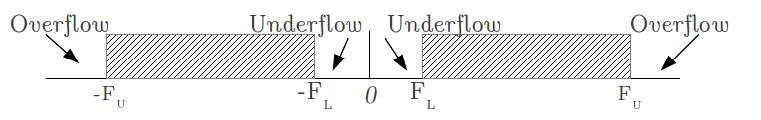
\includegraphics[scale=0.4]{./conj_F.jpg}
  \end{center}
  \caption{N\'umeros de punto flotante $\mathbb{F}(\beta, t, L, U )$.}
  \label{nums_flot}
  \end{figure}  
\end{frame}
%%%%%
\begin{frame}
\frametitle{Forma Normalizada de un N\'umero}
Sea el conjunto de punto flotante $\mathbb{F}$ con par\'ametros $\beta=2$(Binario), $t =3$ , $L = -2$, $U
=2$. Tal conjunto F tiene
$$
2(2-1)2^3-1(2-(-2)+1)+1=41
$$
n\'umeros diferentes (incluyendo el cero), en este caso, las mantisas ser\'ian $(0.100)_2$, $(0.101)_2$, $(0.110)_2$ y
$(0.111)_2$ los cuales son la representaci\'on en base dos de los n\'umeros reales $\frac{1}{2}$, $\frac{5}{8}$,
$\frac{3}{4}$ y $\frac{7}{8}$ respectivamente, el total de n\'umeros de m\'aquina aparecen en la siguiente tabla
\end{frame}
%%%%%
\begin{frame}
\begin{table}[!ht]
  \scriptsize{
\begin{center}
  \begin{tabular}{|c||c||c||c||c|}\hline
  -2  & -1 & 0 & 1 & 2\\\hline\hline
  $(0.100)_2\times2^{-2}$ & $(0.100)_2\times2^{-1}$ & $(0.100)_2\times2^{0}$ & $(0.100)_2\times2^{1}$ &
$(0.100)_2\times2^{2}$\\\hline
  $(0.101)_2\times2^{-2}$ & $(0.101)_2\times2^{-1}$ & $(0.101)_2\times2^{0}$ & $(0.101)_2\times2^{1}$ &
$(0.101)_2\times2^{2}$\\\hline
  $(0.110)_2\times2^{-2}$ & $(0.110)_2\times2^{-1}$ & $(0.110)_2\times2^{0}$ & $(0.110)_2\times2^{1}$ &
$(0.110)_2\times2^{2}$\\\hline
  $(0.111)_2\times2^{-2}$ & $(0.111)_2\times2^{-1}$ & $(0.111)_2\times2^{0}$ & $(0.111)_2\times2^{1}$ &
$(0.111)_2\times2^{2}$\\\hline
 \end{tabular}
 \caption{N\'umeros binarios de $\mathbb{F}(2,3,-2,2)$}\end{center}}
\end{table}
\end{frame}
%%%%%
\begin{frame}
\frametitle{Forma Normalizada de un N\'umero}
\begin{itemize}
 \item<1-> Los 41 n\'umeros de m\'aquina de este conjunto son los siguientes:
 $$
 \begin{array}{l}
 \displaystyle 0, \pm\frac{4}{32}, \pm\frac{5}{32}, \pm\frac{6}{32}, \pm\frac{7}{32}, \pm\frac{8}{32}, \pm\frac{10}{32},
 \pm\frac{12}{32}, \pm\frac{14}{32}, \pm\frac{16}{32}, \pm\frac{20}{32}, \pm\frac{24}{32},
 \pm\frac{28}{32},\\ 
 \displaystyle\pm\frac{32}{32}, \pm\frac{40}{32}, \pm\frac{48}{32}, \pm\frac{56}{32}, \pm\frac{64}{32},
 \pm\frac{80}{32}, \pm\frac{96}{32},  \pm\frac{112}{32}
 \end{array}
 $$
 
 \begin{figure}[ht]
 \begin{center}
   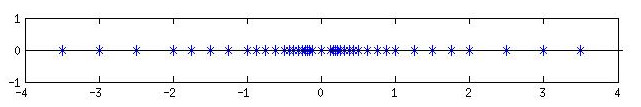
\includegraphics[scale=0.45]{./conj_F_ejem.jpg}
 \end{center}
 \caption{N\'umeros de punto flotante $\mathbb{F}(2, 3, -2, 2 )$.}
 \label{nums_flot_recta_real}
 \end{figure}
\end{itemize}
\end{frame}
%%%%%
\begin{frame}
  \frametitle{Forma Normalizada de un N\'umero}
  \begin{itemize}
   \item<1-> La combinaci\'on aritm\'etica usual $+$, $-$, $\times$, $\div$ de dos n\'umeros de punto flotante no siempre produce un n\'umero de punto flotante. 
   \item <2-> Supongamos que $fl(x)$, $fl(y) \in \mathbb{F}$. Veamos, como ejemplo, que la suma usual
   $fl(x)+fl(y)$ no necesariamente ser\'a un n\'umero en $\mathbb{F}$. Sea el conjunto $\mathbb{F}$ dado en el ejemplo: $fl(x) =5/32 \in \mathbb{F}$, $fl(y) =48/32 \in \mathbb{F}$, sin embargo $fl(x)+fl(y) =
   5/32 + 48/32 = 53/32 \notin \mathbb{F}$.
   \item Las operaciones aritm\'eticas que realiza un computador no corresponden de forma exacta con las operaciones usuales. El estudio de lo que ocurre realmente es dif\'icil de realizar y en todo caso depende de la m\'aquina que se est\'e
   utilizando.
  \end{itemize}
\end{frame}
%%%%%
\begin{frame}
   \frametitle{Forma Normalizada de un N\'umero}
   \begin{itemize}   
   \item Denotando por $\oplus,\ominus,\otimes,\oslash$ las operaciones de suma, resta, multiplicaci\'on y divisi\'on de la m\'aquina. Se definen estas operaciones por:
   \begin{block}{} 
   $$
   \begin{array}{lll}
    x \oplus y & = & fl(fl(x) + fl(y))\\
    x \ominus y & = & fl(fl(x) - fl(y))\\
    x \otimes y & = & fl(fl(x) \times fl(y))\\
    x \oslash y & = & fl(fl(x) / fl(y))\\
   \end{array}
   $$
   \end{block}
   \end{itemize}
\end{frame}
%%%%
\frame{
\frametitle{Ejercicios:}
 Asumiendo $\beta = 10$, $t = 3$, $L = -3$, $U = 4$, y la aritm\'etica es truncada. Obtener los 
valores de:
 
 \begin{itemize}
  \item $fl(0.00009)$
  \item $fl(3.146)$
  \item $fl(9996)$
  \item $fl((100.0 + 0.61) + 0.61)$ y $fl(100.0 + (0.61 + 0.61))$
  \item $fl(2.34 \times (5.67 + 8.90))$ y $fl((2.34 \times 5.67) + (2.34 \times 8.90))$
 \end{itemize}
}
%%%%%%
\frame
{
  \frametitle{Unidad de Precisi\'on o Redondeo} 
  \begin{itemize}
    \item<1-> En la representaci\'on en punto flotante con $n$ d\'igitos en base $\beta$ y exponente $e$, el error relativo en la
    representaci\'on de un n\'umero real $x$, $x\neq0$ es estimado por:     
    $$
    \left|\frac{x-fl(x)}{x}\right|\leq \mu = \left\{\begin{array}{ll}
      \beta^{1-n} & \mbox{ si se trunca}\\
      \frac{1}{2}\beta^{1-n} & \mbox{ si se redondea}
      \end{array}
    \right.
    $$     
    \item<2->El n\'umero $\mu$ (error de redondeo unitario) es una caracter\'istica de la m\'aquina, de su sistema operativo y de la manera en que efect\'ua los c\'alculos. 
    \item<3-> El \'epsilon de la m\'aquina es importante porque caracteriza la precisi\'on de la m\'aquina, sirve adem\'as como criterio de parada de los algoritmos.
  \end{itemize}
}
%%%%%
\begin{frame}
  \frametitle{Unidad de Precisi\'on o Redondeo} 
  \begin{itemize}
    \item Otra definici\'on de $\mu \approx \epsilon$ (\'Epsilon de la m\'aquina): $\epsilon$ es el m\'as peque\~no n\'umero positivo de la forma $\epsilon = 2^{-k}$ tal que:
    $$
    1.0 + \epsilon \neq 1.0 \mbox{  en la m\'aquina}
    $$
    \item<2-> $\epsilon = 2^{-n}$ donde $n$ es la precisi\'on de la m\'aquina. Lo que sucede es que en la aritm\'etica de la m\'aquina llega un momento en que:    
    $$
    fl(1.0 + 2^{-k}) = 1.0
    $$    
  \end{itemize}
\end{frame}
%%%%
\frame
{
  \frametitle{Unidad de Presici\'on o Redondeo.}
  Algoritmo para calcular $\epsilon$
  \begin{itemize}
  \item<1->[1.] $s=1$
  \item<2->[2.] para $k=1,2,\ldots,100$ hacer
  \item<3->[3.] \qquad $s= s*0.5$
  \item<4->[4.] \qquad $t=s+1.0$
  \item<5->[5.] \qquad si ($t<=1.0$) entonces
  \item<6->[6.] \qquad\qquad $s=2.0*s$
  \item<7->[7.] \qquad\qquad salida($k-1$,$s$)
  \item<8->[8.] \qquad\qquad parar
  \item<9->[9.] \qquad fsi
  \item<10->[10.] fpara
  \end{itemize}
}
%%%%%
\section{Propagaci\'on del Error.}
\frame
{
  \frametitle{Propagaci\'on del Error.}
  \begin{itemize}
    \item<1-> Es importante estudiar la propagaci\'on del error en los c\'alculos, ya que los errores se propagan y amplifican al realizar operaciones con dichos datos, hasta el punto de que puede suceder que el resultado carezca de significado.
    \item<2-> Con el proposito de ilustrar esta situaci\'on, seguidamente se calcula la diferencia entre los n\'umeros
    $$
    \begin{array}{l}
     a= 0.276435\\
    b=0.2756
    \end{array}
    $$
    \uncover<3->{Si los c\'alculos se realizan en base diez, punto flotante, redondeo correcto a tres d\'igitos de mantisa, los valores aproximados a dichos n\'umeros y el error relativo cometido es
    $$
    \begin{array}{lcl}
     \tilde a= 0.276 &  & |r_a|=1.57\times10^{-3}\\
    \tilde b=0.276 &  & |r_b|=1.45\times10^{-3}
    \end{array}
    $$}
  \end{itemize}
}
%%%%
\frame
{\frametitle{Propagaci\'on del Error}
\begin{itemize}
  \item Si ahora se calcula la diferencia entre los valores exactos y la diferencia entre los aproximados se obtiene
  $$
  \begin{array}{l}
   a-b= 0.000835\\
  \tilde a-\tilde b=0.0
  \end{array}
  $$
  \uncover<2->{
  \item<2->Debe observa que el error relativo de la diferencia aproximada es del 100\%. Este ejemplo, extraordinariamente sencillo, pone de manifiesto como el error de redondeo de los datos se ha amplificado al realizar una \'unica operaci\'on, hasta generar un resultado carente de significado.
  }
\end{itemize}
}
%%%%
\frame
{
\frametitle{Propagaci\'on del Error en la Suma}

Denotando por $x$ e $y$ los valores exactos de dos n\'umeros y por $\tilde x$ e $\tilde y$ sus valores aproximados. As\'i mismo, los errores absolutos y relativos de estas cantidades se denotar\'an por $E_x$, $E_y$, $r_x$, $r_y$, respectivamente. Si se representa por $s = x + y$ al valor exacto de la suma y por $\tilde s = \tilde x + \tilde y$ su valor aproximado, entonces el error absoluto de la suma es
$$
E_s = s -\tilde s = (x + y) - (\tilde x + \tilde y) = E_x + E_y
$$

El error relativo vale
$$
r_s = \frac{E_s}{s} = \frac{E_x+E_y}{x+y} = \frac{x}{x+y}r_x + \frac{y}{x+y}r_y
$$
}

\frame
{
\frametitle{Propagaci\'on del Erroren la Resta}

La deducci\'on para la propagaci\'on del error mediante la resta es muy parecida a la anterior. Si se representa por $r = x - y$ al valor exacto de la resta y por $\tilde r =\tilde x -\tilde y$ su valor aproximado, entonces el error absoluto es
$$
E_r = r -\tilde r = (x - y) - (\tilde x - \tilde y) = E_x - E_y
$$

El error relativo vale
$$
r_r = \frac{E_r}{r} = \frac{E_x-E_y}{x-y} = \frac{x}{x-y}r_x - \frac{y}{x-y}r_y
$$
}
%%%%
\frame
{
\frametitle{Propagaci\'on del Error en el Producto}
Si se representa el producto de dos n\'umeros exactos mediante $p = xy$ y el valor aproximado del producto por $\tilde p = \tilde x\tilde y$, el error absoluto del producto se puede calcular como

\begin{eqnarray}
\nonumber E_p &=& p -\tilde p = (xy) - (\tilde x \tilde y) = xy - (x-E_x) (y- E_y)\\
\nonumber &=& x E_y + y E_x - E_x E_y \approx xE_y + yE_x
\end{eqnarray}


El error relativo vale
$$
r_p = \frac{E_p}{p} = \frac{xE_y+yE_x-ExEy}{xy} = r_x+r_y+r_xr_y \approx r_x+r_y
$$
}
%%%%
\frame
{
\frametitle{Propagaci\'on del Error en la Divisi\'on}

Si se representa el cociente de dos n\'umeros exactos mediante $d = x/y$ y el valor aproximado del producto por $\tilde d = \tilde x/\tilde y$, el error absoluto del cociente se puede calcular como

\begin{eqnarray}
\nonumber E_d &=& d -\tilde d = \frac{x}{y} - \frac{\tilde x}{\tilde y} =\frac{x}{y} - \frac{x-Ex}{y-Ey}\\
\nonumber &=& \frac{yE_x-xE_y}{y(y-Ey)} \approx \frac{yE_x-xE_y}{y^2}
\end{eqnarray}


El error relativo vale
$$
r_d = \frac{E_d}{d} = \frac{\frac{yE_x-xE_y}{y(y-Ey)}}{\frac{x}{y}} = \frac{yE_x-xE_y}{x(y-E_y)} =  \frac{r_x-r_y}{1-r_y} \approx r_x-r_y
$$
}
%%%%
\frame
{
\frametitle{Propagaci\'on del Error en una Funci\'on}

Sea $z = f(x)$ la imagen mediante la funci\'on $f$ del valor exacto de un n\'umero $x$ y sea $\tilde z = f(\tilde x)$ la imagen de su valor aproximado. Entonces, el error absoluto de la imagen es

\begin{eqnarray}
\nonumber E_z &=& f(x) -f(\tilde x) = f(x) - f(x-E_x)\\
\nonumber &=& f(x) - \left[f(x)-f'(x)E_x+f''(x)\frac{E_x^2}{2!}-f'''(x)\frac{E_x^3}{3!}+\cdots\right]\\
\nonumber &=& f'(x)E_x-f''(x)\frac{E_x^2}{2!}+f'''(x)\frac{E_x^3}{3!}-\cdots \approx f'(x)E_x
\end{eqnarray}


El error relativo vale
%\small 
$$
r_z = \frac{E_z}{z} = \frac{f'(x)E_x-f''(x)\frac{E_x^2}{2!}+f'''(x)\frac{E_x^3}{3!}-\cdots}{f(x)}  \approx  x\frac{f'(x)}{f(x)}r_x 
$$
}








% \frame
% {
%   \frametitle{Motivaci\'on.} 
%   \begin{itemize}
%    \item<1->La formulaci\'on de problemas de ingenier\'ia a menudo conduce a sistemas lineales de ecuaciones. Estos sistemas pueden llegar a tener cientos o miles de grados de libertad. 
%    \item<2-> El objetivo de este tema es desarrollar estrategias num\'ericas que permitan resolver sistemas de ecuaciones relativamente grandes de una manera eficiente. 
%    \item<3-> Adem\'as, se analizar\'an con detalle algunos m\'etodos directos.
%   \end{itemize}
% }
% %%%%
% \frame
% {
%    \frametitle{Motivaci\'on.}
   
% Si bien existen m\'etodos exactos  como el m\'etodo de Cramer, estos son muy costosos de aplicar en situaciones donde los sistemas a resolver tienen muchas ecuaciones.

% El n\'umero total de operaciones para resolver un sistema de dimensi\'on $n$ con este m\'etodo es
% $$
% T_C = (n+1)^{2}n!-1
% $$

% \begin{table}[!ht]
%  \begin{tabular}{|c|c|}\hline
% $n$ & $T_C$  \\\hline
% $5$ & $4319$ \\\hline
% $10$ & $4\times10^8$\\\hline
% $100$ &  $10^{158}$\\\hline
%  \end{tabular}
% \caption{Operaciones elementales del m\'etodo de Cramer segun el tama\~no de la matriz($n$).}
% \end{table}
% }
% %%%%
% \frame{
% \frametitle{Motivaci\'on.}
% Desde el punto de vista num\'erico se buscan algoritmos eficientes en diferentes aspectos:
% \begin{itemize}
%  \item<2-> N\'umero de operaciones necesarias (tiempo CPU)
%  \item<3-> Necesidades de almacenamiento (memoria)
%  \item<4-> Rango de aplicabilidad (sobre que tipo de matrices se pueden aplicar)
% \end{itemize}
% }
% %%%%%
% \frame
% {
% \frametitle{Introducci\'on.}
% Un sistema de $n$-ecuaciones (con coeficientes reales) en las $n$-inc\'ognitas $x_1,
% x_2,\ldots,x_n$ es un conjunto de $n$ ecuaciones de la forma:

% $$
% \left\{
% \begin{array}{c}
%   f_1(x_1,x_2,\ldots,x_n)=0 \\
%   f_2(x_1,x_2,\ldots,x_n)=0 \\
%   \dotfill \\
%   f_n(x_1,x_2,\ldots,x_n)=0 \\
% \end{array}
% \right.
% $$

% donde
% $$f_i(x_1,x_2,\ldots,x_n) = a_{i,1}x_1 + a_{i,2}x_2 + \cdots + a_{i,n}x_n - b_i$$
% }
% %%%
% \frame
% {
% con $a_{i,1},a_{i,2},\ldots,a_{i,n}$ y $b_i$ constantes reales, el sistema se dice lineal (con coeficientes reales);
% en cualquier otro caso el sistema se dice no-lineal.

% \vspace{0.5cm}
% \uncover<2->{
%   A los n\'umeros $a_{ij}$ se les denomina coeficientes del sistema y a los $b_i$ t\'erminos independientes.  
% }

% \vspace{0.5cm}
% \uncover<3->{
% Si $C = (c_1, c_2,\ldots,c_n) \in \mathbb{R}^n$ es tal que $f_i(c_1,c_2,\ldots,c_n) = 0$ para cada $i = 1,2,\ldots,n$,
% entonces se dice que $C$ es una soluci\'on real del sistema planteado.
% }}
% %%%%
% \frame{
% Si se introducen las matrices
% $$
%   A = \left[\begin{array}{cccc}
%             a_{11} & a_{12} & \cdots & a_{1n}\\
%             a_{21} & a_{22} & \cdots & a_{2n}\\
%             \vdots & \vdots & \ddots & \vdots\\
%             a_{m1} & a_{m2} & \cdots & a_{mn}\\
%         \end{array}\right], \qquad x=\left[\begin{array}{c}
%           x_1\\
%           x_2\\
%           \vdots\\
%           x_n\\
%         \end{array}\right], \qquad b=\left[\begin{array}{c}
%           b_1\\
%           b_2\\
%           \vdots\\
%           b_m\\
%         \end{array}\right]
% $$

% el sistema se puede representar de forma m\'as compacta por
% $$
% Ax=b
% $$
% }
% %%%%
% \frame{
%   Podemos clasificar los sistemas de ecuaciones lineales atendiendo a:
%   \begin{enumerate}
%     \item Su tama\~no
%       \begin{enumerate}
%         \item Peque\~nos: $n \leq 300$ donde $n$ representa el n\'umero de ecuaciones.
%         \item Grandes: $n>300$
%       \end{enumerate}
%     \item<2-> Su estructura
%       \begin{enumerate}
%         \item Si la matriz posee pocos elementos nulos diremos que se trata de un sistema lleno.
%         \item Si, por el contrario, la matriz contiene muchos elementos nulos, diremos que la matriz, y por lo tanto, el sistema lineal es disperso o \textit{sparce}.
%       \end{enumerate}
% \end{enumerate}
% }
% \frame{
%   \begin{enumerate}
%   \item Matrices de este tipo son las denominadas
%       \begin{itemize}
%         \item Tridiagonales
%           $$
%           \left(\begin{array}{cccc}
%             a_{1,1} & a_{1,2} & 0 & 0 \\
%             a_{2,1} & a_{2,2} & a_{2,3} & 0 \\
%             0 & a_{3,2} & a_{3,3} & a_{3,4} \\
%             0 & 0 & a_{4,3} & a_{4,4} \\
%             \end{array}\right)
%           $$
%       \item<2-> Triangulares Superiores
%           $$
%           \left(\begin{array}{cccc}
%             a_{1,1} & a_{1,2} & a_{1,3} & a_{1,4} \\
%             0 & a_{2,2} & a_{2,3} & a_{2,4} \\
%             0 & 0 & a_{3,3} & a_{3,4} \\
%             0 & 0 & 0 & a_{4,4} \\
%             \end{array}\right)
%           $$
%       \item<3-> Triangulares Inferiores
%           $$
%           \left(\begin{array}{cccc}
%             a_{1,1} & 0 & 0 & 0 \\
%             a_{2,1} & a_{2,2} & 0 & 0 \\
%             a_{3,1} & a_{3,2} & a_{3,3} & 0 \\
%             a_{4,1} & a_{4,2} & a_{4,3} & a_{4,4} \\
%             \end{array}\right)
%           $$
%     \end{itemize}
%    \end{enumerate} 
% }
% %%%%
% \frame{
% \frametitle{Existencia y unicidad de soluciones}
% \begin{block}{Teorema: Compatibilidad de un sistema de ecuaciones lineales}
%   La ecuaci\'on $Ax=b$ admite soluci\'on si y s\'olo si
%   $$
%   rango(A|b) = rango(A)
%   $$
% \end{block}

% \uncover<2->{
% \begin{block}{Corolario}
%  Si $A^{m\times n}$ tiene rango $m$, $Ax=b$ siempre tiene soluci\'on
% \end{block}}

% \uncover<3->{
% \begin{block}{Teorema}
%   Si $x_0$ es una soluci\'on de $Ax=b$, el conjunto de soluciones de la ecuaci\'on est\'a dado por $x_0+ker(A)$.
% \end{block}}

% \uncover<4->{
% \begin{block}{Corolario}
%  Una soluci\'on de $Ax=b$ es \'unica si y s\'olo si $ker(A)=\emptyset$.
% \end{block}}
% }
% %%%%
% \frame{
% \frametitle{Existencia y unicidad de soluciones}
% Consid\'erese una matriz cuadrada $A \in \mathbb{R}^{n\times n}$. Las siguientes condiciones son equivalentes:
% \begin{itemize}
%  \item<2-> Para cualquier $b \in \mathbb{R}^{n}$ el sistema $Ax=b$  tiene soluci\'on.
%  \item<3-> Si $Ax=b$ tiene soluci\'on, \'esta es \'unica.
%  \item<4-> Para cualquier $x \in \mathbb{R}^{n}$, $Ax=0 \Rightarrow x=0$.
%  \item<5-> Las columnas (filas) de la matriz $A$ son linealmente independientes.
%  \item<6-> Existe una matriz cuadrada $A^{-1}$ (matriz inversa) tal que
%  $$
%  AA^{-1} = A^{-1}A = I
%  $$
%  \item<7-> La matriz $A$ tiene determinante no nulo
%  $$
%  |A| = \det(A) \neq 0
%  $$
% \end{itemize}
% }
% %%%%%
% \frame{
% La primera opci\'on que se plantea es
% $$
% x = A^{-1}b
% $$
% \begin{itemize}
%  \item<2-> No es eficiente (demasiadas operaciones).
%  \item<3-> Si el determinante de $A$ es pr\'oximo a cero, el error de redondeo puede ser muy grande, y esto es dificil de estimar num\'ericamente
%  $$
%  \det(\gamma A) = \gamma^{n}\det(A)
%  $$
% \end{itemize}
% }
% %%%%
% \frame{
% Se requieren m\'etodos num\'ericos alternativos
% \begin{itemize}
%  \item<2-> m\'etodos directos, son exactos (no tienen asociado error de truncamiento), y son usados 
% cuando la mayor\'ia de los coeficientes de $A$ son distintos de cero y las matrices no son demasiado 
% grandes. Suelen ser algoritmos ``complicados de implementar''
%  \item<3-> m\'etodos indirectos o iterativos, tienen asociado un error de truncamiento y se usan 
% preferiblemente para matrices grandes ($n>>1000$) cuando los coeficientes de $A$ son la mayor\'ia 
% nulos (matrices sparse). Algoritmos sencillos de implementar que requiere aproximaci\'on inicial y 
% que en general no tiene porqu\'e converger (requieren an\'alisis de convergencia previo).
% \end{itemize}

% }
% \section{M\'etodos Directos}
% \begin{frame}
%   \frametitle{M\'etodos Directos}
%   \begin{itemize}
%     \item \underline{\textbf{CASO 1}}: La matriz $A$ de coeficientes del sistema $Ax = b$ es triangular (superior o inferior) con
%     todas sus componentes sobre la diagonal principal no nulas.
    
%     $$
%     \left\{\begin{array}{rcc}
%             a_{1,1}x_1 + a_{1,2}x_2 + \cdots + a_{1,i}x_i + \cdots + a_{1.n}x_n & = & b_1\\
%              a_{2,2}x_2 + \cdots + a_{2,i}x_i + \cdots + a_{2,n}x_n & = & b_2\\
%               \vdots & & \vdots\\
%                  a_{i,i}x_i + \cdots + a_{i,n}x_n & = & b_i\\
%                         \vdots & & \vdots\\
%                      a_{n,n}x_n & = & b_n\\
%            \end{array}\right.
%     $$
%   \end{itemize}
% \end{frame}
% %%%%%
% \frame{
%   Como $a_{n,n} \neq 0$, se puede despejar $x_n$ de la \'ultima ecuaci\'on, y se obtiene:
%   $$
%   x_n = \frac{b_n}{a_{n,n}}
%   $$
%   conocido el valor de $x_n$, se puede emplear la pen\'ultima ecuaci\'on para conocer $x_{n-1}$
%   $$
%   x_{n-1} = \displaystyle\frac{b_{n-1}-a_{n-1,n}x_n}{a_{n-1,n-1}}
%   $$
%   conocidos $x_n$ y $x_{n-1}$, se obtiene de la antepen\'ultima ecuaci\'on
%   $$
%   x_{n-2} = \displaystyle\frac{b_{n-2}-\left(a_{n-2,n-1}x_{n-1}+a_{n-2,n}x_{n}\right)}{a_{n-2,n-2}}
%   $$
% }
% %%%%%
% \frame{
%   En general, conocidos $x_n, x_{n-1},\ldots,x_{i+1}$, se obtiene:
%   $$
%   x_i =  \frac{b_i - \displaystyle\sum_{k=i+1}^na_{i,k}x_k}{a_{i,i}} \quad\,\,\,\, \forall i=n-1,n-2,\ldots,2,1
%   $$
%   El m\'etodo anterior para determinar la soluci\'on del sistema se denomina sustituci\'on regresiva o hacia atr\'as.  
% }
% %%%
% \begin{frame}
%   Si la matriz de coeficientes del sistema es triangular inferior, para resolver el sistema podemos proceder de manera similar al caso anterior, pero empezando por despejar $x_1$ de la primera ecuaci\'on. El procedimiento en este caso se denomina sustituci\'on progresiva o hacia adelante.
%   $$
%     \left\{\begin{array}{lcc}
%             a_{1,1}x_1  & = & b_1\\
%             a_{2,1}x_1 + a_{2,2}x_2 & = & b_2\\
%               \vdots & & \vdots\\
%             a_{i,1}x_1 + \cdots + a_{i,i-1}x_{i-1} + a_{i,i}x_i  & = & b_i\\
%             \vdots & & \vdots\\
%             a_{n,1}x_{1} + a_{n,2}x_2 + \cdots + a_{n,i-1}x_{i-1} + a_{n,i}x_i + \cdots + a_{n,n}x_n & = & b_{n}
%            \end{array}\right.
%     $$
% \end{frame}
% %%%%
% \frame{
%   \begin{itemize}
%     \item \underline{\textbf{CASO 2}}: La matriz $A$ de coeficientes, del sistema lineal $Ax = b$, es tal que no se requieren
%     intercambios de
%     filas para culminar con \'exito la eliminaci\'on Gaussiana.
    
%     Digamos que el sistema $Ax = b$ tiene la forma
%     $$
%     \left\{\begin{array}{cccc}
%       E_1: & a_{1,1}x_1 + a_{1,2}x_2 + \cdots + a_{1,j}x_j + \cdots + a_{1,n}x_n & = & b_1\\
%       E_2: & a_{2,1}x_1 + a_{2,2}x_2 + \cdots + a_{2,j}x_j + \cdots + a_{2,n}x_n & = & b_2\\
%       & \vdots &   &\\
%       E_j: & a_{j,1}x_1 + a_{j,2}x_2 + \cdots + a_{j,j}x_j + \cdots + a_{j,n}x_n & = & b_j\\
%       & \vdots &   &\\
%       E_i: & a_{i,1}x_1 + a_{i,2}x_2 + \cdots + a_{i,j}x_j + \cdots + a_{i,n}x_n & = & b_i\\
%       & \vdots &   &\\
%       E_n: & a_{n,1}x_1 + a_{n,2}x_2 + \cdots + a_{n,j}x_j + \cdots + a_{n,n}x_n & = & b_n\\
%       \end{array}\right.
%     $$
%   \end{itemize}
% }
% %%%%%
% \frame{
%   El proceso de eliminaci\'on Gaussiana sin Pivoteo consiste en lo siguiente:
% \begin{enumerate}
%  \item<2-> Se elimina el coeficiente de $x_1$ en cada una de las ecuaciones $E_2,E_3,\ldots,E_n$ para obtener un sistema
% equivalente $A^{(1)}x=b^{(1)}$, realizando las operaciones elementales
% $$
% \left(E_i - \left(\frac{a_{i,1}}{a_{1,1}}\right)E_1\right)\rightarrow E_i^{(1)}, \quad \forall\,\,\, i=2,3,\ldots,n
% $$
%   \item<3-> Se elimina el coeficiente de $x_2$ en cada una de las ecuaciones $E_3^{(1)},E_4^{(1)},\ldots,E_n^{(1)}$, para
% obtener un sistema equivalente $A^{(2)}x=b^{(2)}$, realizando las operaciones elementales
% $$
% \left(E_i^{(1)} - \left(\frac{a_{i,2}^{(1)}}{a_{2,2}^{(1)}}\right)E_2^{(1)}\right)\rightarrow E_i^{(2)}, \quad
% \forall\,\,\, i=3,4,\ldots,n
% $$  
% \end{enumerate}
% }
% %%%%%
% \frame{
% \begin{enumerate}
%   \item En general, eliminados los coeficientes de $x_1,x_2,\ldots,x_{j-1}$, se elimina el coeficiente de $x_j$ en cada
%   una de las ecuaciones, para obtener un sistema equivalente $A^{(j)}x=b^{(j)}$, realizando las operaciones elementales
%   $$
%   \left(E_i^{(j-1)} - \left(\frac{a_{i,j}^{(j-1)}}{a_{j,j}^{(j-1)}}\right)E_j^{(j-1)}\right)\rightarrow E_i^{(j)}, \quad
%   \forall\,\,\, i=j+1,\ldots,n
%   $$
%   debe ocurrir que $a_{j,j}\neq 0$.
% \end{enumerate}
% }
% %%%%%
% \frame{
%   Los n\'umeros
% $$
% m_{i,j} = \frac{a_{i,j}^{(j-1)}}{a_{j,j}^{(j-1)}}\quad \forall\,\,\, j=1,\ldots,n-1,\,\, i=j+1,\ldots,n
% $$
% se llaman multiplicadores.

% El sistema resultante tendr\'a entonces la forma triangular superior con elementos no nulos en la diagonal, por lo tanto, se puede resolver mediante sustituci\'on regresiva.
% }
% %%%%
% \frame{
% \begin{algorithm}[H]
% % \SetLine
%  \SetKwInOut{Input}{input}
%  \SetKwInOut{Output}{output}
%  \caption{Algoritmo de eliminaci\'on Gaussiana sin pivoteo.}
%  \Input{$A \in \mathbb{R}^{n \times n}$, $b \in \mathbb{R}^n$}
%  \Output{Matriz $A \in \mathbb{R}^{n \times n}$ tal que $A$ es triangular superior.}
%  \BlankLine
%  \For{$k\leftarrow 1$ \KwTo $n-1$}
%  {
%    \For{$i\leftarrow k+1$ \KwTo $n$}
%     {
%       $factor \leftarrow \displaystyle\frac{a_{i,k}}{a_{k,k}}$\\
%       $a_{i,k} \leftarrow 0$\\
%       \For{$j \leftarrow k+1$ \KwTo $n$}
%       {
%         $a_{i,j} \leftarrow a_{i,j}-factor*a_{k,j}$\\
%       }	
%       $b_i \leftarrow b_i-factor*b_k$\\
%   }
%  }
% \end{algorithm}
% }
% %%%%
% \frame{
%   Utilice la eliminaci\'on Gaussiana sin pivoteo para resolver el sistemas de ecuaciones.
%   $$
% \left\{\begin{array}{l}
%     2x_1 + x_2 + x_3 = -3\\
%     x_1 - 2x_2 + 3x_3 = 6\\
%     x_1 - x_2 - x_3 = 6\\
%     \end{array}\right.
%   $$
% }
% %%%%
% \section{Estrategias de Pivoteo}
% \begin{frame}
%   \frametitle{Pivoteo Parcial}
%   Ejemplo de la necesidad de pivoteo parcial, en una aritm\'etica de 4 d\'igitos con redondeo correcto
% $$
% \left\{\begin{array}{l}
%         0.003000x_1 + 59.14x_2 = 59.17\\
% 	5.291x_1-6.130x_2=46.78\\
%        \end{array}\right.
% $$

% cuya soluci\'on exacta es $x_1=10,00$ y $x_2=1,000$.

% \end{frame}
% %%%%
% \begin{frame}
% \frametitle{Pivoteo Parcial}
% \begin{itemize}
%   \item Si se realizan los pasos de eliminaci\'on Gaussiana se obtiene el siguiente resultado $\tilde{x}_1 = -10,00$ y $\tilde{x}_2=1,001$, el cual difiere bastante de la soluci\'on real, en el valor $x_1$.

%   \item<2-> El error tan grande de la soluci\'on num\'erica de $x_1$, resulta del error peque\~no de $0,001$ al resolver para $x_2$.
% \end{itemize}
  
% \end{frame}
% %%%%
% \begin{frame}
% \frametitle{Pivoteo Parcial}
% \begin{itemize}
%   \item<1-> Ahora, si se elige como pivote
%   el m\'aximo entre $a_{1,1}$ y $a_{2,1}$.
  
%   \item<2-> Pivote =$ \max(|0.003|;|5.291|)=5.291$, por tanto se realiza un intercambio de filas quedando el sistema de la siguiente manera:
%   $$
%   \left\{\begin{array}{l}
%     5.291x_1-6.130x_2=46.78\\
%           0.003000x_1 + 59.14x_2 = 59.17\\
%          \end{array}\right.
%   $$
%   \item<3-> cuya soluci\'on aproximada es $\tilde x_2 = 1 = x_2$ y  $\tilde x_1 = 10 = x_1$.
%   \end{itemize}
% \end{frame}
% %%%%%
% \begin{frame}
% \frametitle{Pivoteo Parcial}
% \begin{itemize}
%   \item<1-> Por tanto para cada paso de eliminaci\'on gaussiana tenemos que:
%   \begin{block}{EGPP}
%       $$
%         \mbox{Paso }k\left\{\begin{array}{l}
%             \mbox{Elegir }p\mbox{ como el primero tal que}\\
%             |a_{p,k}^{(k-1)}|=\max|a_{i,k}^{(k-1)}|\,\,\,k\leq i\leq n
%             \end{array}\right.
%       $$  
%   \end{block}  
% \end{itemize}
% \end{frame}
% %%%%
% \begin{frame} 
% \frametitle{Pivoteo Parcial}
% \begin{itemize}
%   \item<1-> Sea el Sistema lineal 
%   $$
%   \left(\begin{array}{cc|c}
%          1 & 10^4 & 10^4 \\
%          1 & 10^{-4} & 1 \\
%         \end{array}
%   \right)
%   $$
%   \item<2-> Soluci\'on exacta con 4 decimales correctos $x_1 = x_2 = 0.9999$.  
%   \item<3-> No hay pivoteo, ya que $|a_{1,1}|=|a_{2,1}|$. Se obtiene $\tilde x_2=1$ y $\tilde x_1=0$.
% \end{itemize}
% \end{frame}
% %%%%%
% \begin{frame}
% \frametitle{Pivoteo Escalado}
% \begin{itemize}
%   \item<1-> Si se realiza pivoteo escalado de la siguiente manera.
%   \item <2-> se busca el m\'aximo por fila y luego se divide cada fila por dicho factor de escalamiento para luego aplicar pivoteo parcial.
%   \uncover<3->{\begin{eqnarray}
%     \nonumber S_1 = \max(|1|,|10^4|) = 10^4\\
%     \nonumber S_2 = \max(|1|,|10^{-4}|) = 1
%     \end{eqnarray}}  
%   \item<4->se obtiene el siguiente sistema:
%   $$
%   \left(\begin{array}{cc|c}
%          10^{-4} & 1 & 1 \\
%          1 & 10^{-4} & 1 \\
%         \end{array}
%   \right)$$
%   \item<5->y a este nuevo sistema lineal, equivalente al sistema original, se aplica la estrategia de pivoteo parcial.
% \end{itemize}
% \end{frame}
% %%%%
% \frame{
% \frametitle{Pivoteo Completo}
% \begin{itemize}
%   \item<1-> Es otra estrategia de pivoteo en el cual se intercambian filas y columnas en busca del m\'aximo de la matriz y colocarlo como pivote.
%   \item<2->$$
% \left\{\begin{array}{lcl}
%         x_1+10^4x_2 & = & 10^4\\
%         x_1+10^{-4}x_2 & = & 1\\
%        \end{array}
% \right.\equiv \left(\begin{array}{cc|c}
%        1 & 10^4 & 10^4 \\
%        1 & 10^{-4} & 1 \\
%       \end{array}
% \right)
% $$
% \item<3-> $$
% \max(|1|, |10^4|, |1|, |10^{-4}|) \Rightarrow \left(\begin{array}{cc|c}
%        10^4 & 1 & 10^4 \\
%        10^{-4} & 11 & 1 \\
%       \end{array}\right)
% $$
% \end{itemize}
% }
% %%%%
% \frame{
% \frametitle{Pivoteo Completo}
% \begin{itemize}
%   \item<1-> Entonces la estrategia de pivoteo completo consiste en

%   \begin{enumerate}
%    \item $$
%   \mbox{Paso }k\left\{\begin{array}{l}
%           \mbox{elegir }p \mbox{ y }q \mbox{ como los menores tales que}\\
%          \left|a_{p,q}^{(k-1)}\right|=\max\left|a_{i,j}^{(k-1)}\right|\,\,\,k\leq i,j\leq n\\
%                     \end{array}
%   \right.
%   $$
%   \item Intercambiar filas $k$ y $p$.
%   \item Intercambiar columnas $k$ y $q$.
  
%   \end{enumerate}
% \end{itemize}
% }
% %%%%%
% \frame{
% \frametitle{Pr\'actica}
% \begin{itemize}
%   \item Resuelva el siguiente sistema lineal con truncamiento a 5 d\'igitos
%   $$
%   \left\{\begin{array}{l}
%          20x_1 + 15x_2 + 10x_3 = 45 \\
%          -3x_1 - 2.249x_2 + 7x_3 = 1.751 \\
%          5x_1 + x_2 + 3x_3 = 9          
%         \end{array}
%   \right.
%   $$
%   \item Usando Eliminaci\'on Gaussiana sin Pivoteo y luego con las diferentes estrategias de pivoteo compare los resultados obtenidos.
% \end{itemize}
% }
% %%%%%
% \section{Conteo de Operaciones}
% \begin{frame}
%   \frametitle{Conteo de Operaciones}
% \begin{block}{}
%   $$
%   \begin{array}{l}
%     \displaystyle\sum_{i=1}^mcf(i) = c\sum_{i=1}^mf(i) \\
%     \displaystyle\sum_{i=1}^mf(i)+g(i)=\sum_{i=1}^mf(i)+\sum_{i=1}^mg(i)\\
%     \displaystyle\sum_{i=1}^m1=1+1+\cdots+1=m \\ \displaystyle\sum_{i=k}^m1=\sum_{i=k-k+1}^{m-k+1}1=\sum_{i=1}^{m-k+1}1=m-k+1\\
%     \displaystyle\sum_{i=1}^mi=1+2+\cdots+m=\frac{m(m+1)}{2} \\
%     \displaystyle\sum_{i=1}^mi^2=1+4+\cdots+m^2=\frac{m(m+1)(2m+1)}{6}
%     \end{array}
%     $$
% \end{block}  
% \end{frame}
% %%%%
% \begin{frame}
%   \frametitle{Conteo de Operaciones}
%   Dadas estas definiciones, se puede hacer el conteo de operaciones para el algoritmo de eliminaci\'on Gaussiana sin pivoteo.
%   $$
%   \text{Total de Operaciones} = (+/-) + (\times/\div)
%   $$
% \end{frame}
% %%%%%
% %%%%
% \frame{
%   \textbf{Algoritmo de Eliminaci\'on Gaussiana sin Pivoteo.}
% \begin{algorithm}[H]
% % \SetLine
%  \SetKwInOut{Input}{input}
%  \SetKwInOut{Output}{output}
%  %\caption{Algoritmo de eliminaci\'on Gaussiana sin pivoteo.}
%  \Input{$A \in \mathbb{R}^{n \times n}$, $b \in \mathbb{R}^n$}
%  \Output{Matriz $A \in \mathbb{R}^{n \times n}$ tal que $A$ es triangular superior.}
%  \BlankLine
%  \For{$k\leftarrow 1$ \KwTo $n-1$}
%  {
%    \For{$i\leftarrow k+1$ \KwTo $n$}
%     {
%       $factor \leftarrow \displaystyle\frac{a_{i,k}}{a_{k,k}}$\\
%       $a_{i,k} \leftarrow 0$\\
%       \For{$j \leftarrow k+1$ \KwTo $n$}
%       {
%         $a_{i,j} \leftarrow a_{i,j}-factor*a_{k,j}$\\
%       }	
%       $b_i \leftarrow b_i-factor*b_k$\\
%   }
%  }
% \end{algorithm}
% }
% %%%%%
% \begin{frame}
%   \frametitle{Pr\'actica}
%   \begin{itemize}
%    \item Calcular el n\'umero de operaciones en el algoritmo de multiplicaci\'on de dos matrices triangulares superiores.
%    \item Calcular el n\'umero de operaciones en el algoritmo de soluci\'on de una sistema tridiagonal de ecuaciones lineales.
%    \item Calcular el n\'umero de operaciones en el algoritmo de Gauss-Jordan (cuando la matriz del sistema se reduce a la matriz identidad).
%   \end{itemize}
% \end{frame}
% %%%%
% \section{Condicionamiento}
% \frame{
%   \frametitle{Condicionamiento de Sistemas.}
%   \begin{itemize}
%     \item<1-> Sea el sistema lineal $Ax=b$ con
%     \begin{eqnarray}
%      \nonumber A=\left(\begin{array}{cccc}
%                         10 & 7 & 8 & 7\\
%                         7 & 5 & 6 & 5\\
%                         8 & 6 & 10 & 9\\
%                         7 & 5 & 9 & 10\end{array}\right)\\
%      \nonumber b=\left(\begin{array}{c}
%                         32\\
%                         23\\
%                         33\\
%                         31
%                        \end{array}\right)
%     \end{eqnarray}
%     \item<2-> El sistema lineal anterior tiene como soluci\'on un vector de componentes unitarias. 
%     \item<3-> El sistema lineal resultante en realidad no ser\'a ese, sino que ser\'a un sistema lineal perturbado tanto en la matriz del sistema como en el t\'ermino independiente. El sistema lineal perturbado podr\'ia tener el siguiente aspecto.
%     \end{itemize}    
% }
% %%%%
% \frame{
% \frametitle{Condicionamiento de Sistemas.}
% \begin{eqnarray}
%  \nonumber A+\Delta A=\left(\begin{array}{cccc}
%                     10 & 7 & 8.1 & 7.2\\
%                     7.08 & 5.04 & 6 & 5\\
%                     8 & 5.98 & 9.89 & 9\\
%                     6.99 & 4.99 & 9 & 9.98\end{array}\right)\\
%  \nonumber b+\Delta b=\left(\begin{array}{c}
%                     32.01\\
%                     23.02\\
%                     33.03\\
%                     31.04\end{array}\right)
% \end{eqnarray}
% } 
% %%%%
% \frame{
%   y por tanto $\Delta A$ y $\Delta b$, las perturbaciones, tendr\'ian los siguientes valores:

% \begin{eqnarray}
%   \nonumber \Delta A=\left(\begin{array}{cccc}
%                     0 & 0 & 0.1 & 0.2\\
%                     0.08 & 0.04 & 0 & 0\\
%                     0 & -0.02 & -0.11 & 0\\
%                     -0.01 & -0.01 & 0 & -0.02\end{array}\right)\\
%   \nonumber \Delta b=\left(\begin{array}{c}
%                     0.01\\
%                     -0.01\\
%                     0.01\\
%                     -0.01
%                   \end{array}\right)
% \end{eqnarray}
% }
% %%%%
% \frame{
%   \frametitle{Condicionamiento de Sistemas.}
%   \begin{itemize}
%     \item<1-> C\'omo var\'ia la soluci\'on del sistema lineal cuando se perturba la matriz del sistema y cuando se perturba s\'olo el t\'ermino independiente?.
%     \item<2-> Resolviendo primero el sistema lineal:
%     $$
%     A(x + \Delta x) = b + \Delta b
%     $$
    
%     $$
%     x+\Delta x = \left(\begin{array}{c}
%                         1.82\\
%                         -0.36\\
%                         1.35\\
%                         0.79
%                        \end{array}\right) \Rightarrow \Delta x = \left(\begin{array}{c}
%                         0.82\\
%                         -1.36\\
%                         0.35\\
%                         -0.21
%                        \end{array}\right)
%     $$
%     \end{itemize}
% }
% %%%%
% \frame{
%   \frametitle{Condicionamiento de Sistemas.}
%   Se ha perturbado el t\'ermino independiente
% $$
% \frac{\|\Delta b\|_{\infty}}{\|b\|_{\infty}} = 3.03\times10^{-4}
% $$
% y esta perturbaci\'on induce una variaci\'on en la soluci\'on
% $$
% \frac{\|\Delta x\|_{\infty}}{\|x\|_{\infty}} = 1.36
% $$
% }
% %%%%
% \frame
% {
% El sistema est\'a bien condicionado si cuando $\Delta b$ es peque\~na, $\Delta x$ tambi\'en lo es. Observese que:

% \uncover<2->{
% $$
% \left.\begin{array}{ccc}
%  Ax +A(\Delta x) & = & b + \Delta b\\
%  Ax & = & b
% \end{array}\right\}\Rightarrow\left\{\begin{array}{ccc}
%  A(\Delta x) & = & \delta b\\
%  \Delta x & = & A^{-1}(\Delta b)
% \end{array}\right.
% $$
% }

% \uncover<3->{
% Usando la propiedad para normas matriciales:
% $$
% \|\Delta x\| \leq \|A^{-1}\|\|\Delta b\|
% $$
% }

% \uncover<4->{
% De la soluci\'on exacta, $\|b\| \leq \|A\|\|x\|$ , lo que implica que:

% $$
% \frac{1}{\|x\|}\leq\frac{\|A\|}{\|b\|}
% $$
% }
% }
% %%%%
% \frame
% {
% De las dos relaciones anteriores se llega a que:

% $$
% \frac{\|\Delta x\|}{\|x\|} \leq \|A\|\|A^{-1}\|\frac{\|\Delta b\|}{\|b\|}
% $$

% donde $\frac{\|\Delta x\|}{\|x\|}$ representa el error relativo en los resultados, y $\frac{\|\Delta b\|}{\|b\|}$ el error relativo en los datos.

% \uncover<2->{
% De la relaci\'on, parece deducirse que el n\'umero $\|A\|\|A^{-1}\|$ es el factor determinante de la relaci\'on, ya que si es peque\~no se tendr\'a el efecto deseado, y si no, ocurre lo contrario.
% }
% }
% %%%%%
% \frame
% {
% \begin{block}{Definici\'on}
% Sea $\| \cdot \|$ una norma matricial subordinada y $A$ una matriz invertible. Se denomina n\'umero de condici\'on de la matriz $A$ respecto de la norma $\| \cdot \|$ a la expresi\'on:
% $$
% \kappa(A) = \|A\|\|A^{-1}\|
% $$
% \end{block}
% }
% %%%%%
% \frame{
% \begin{itemize}
%  \item Si los datos de un sistema $Ax=b$ son exactos con la precisi\'on de la m\'aquina, el error relativo de la soluci\'on cumple que
%  $$
%  \dfrac{\|x^{*}-x\|}{\|x\|} \leq \kappa(A)\epsilon
%  $$
%  \item<2-> El concepto de n\'umero de condici\'on de una matriz se generaliza a cualquier matriz $A$ (no necesariamente cuadrada) de rango completo mediante la expresi\'on
%  $$
%  \kappa(A) = \|A\|\|A^{\dagger}\|
%  $$
%  donde $A^{\dagger}$ es la matriz pseudoinversa de la matriz $A$.
%  \item<3-> El n\'umero de condici\'on de una matriz $A$ es un indicador del error de amplificaci\'on que produce en un vector $x$ el someterlo a la transformaci\'on que define dicha matriz $A$.
% \end{itemize}

% }
% %%%%%
% \frame{
% \begin{itemize}
%  \item<1-> Estudiando la sensibilidad de un sistema de ecuaciones a peque\~nas perturbaciones en los coeficientes de la matriz.
%  \item<2-> Comparando la soluci\'on de
%  $$
%  Ax=b \qquad \mbox{ y } \qquad (A+\Delta A)(x+\Delta x)=b
%  $$
%  \item<3-> De la segunda igualdad, como $Ax=b$, haciendo $\Delta x = -A^{-1}\Delta A(x+\Delta x)$, despreciando el producto $\Delta A\cdot\Delta x$, resulta que
%  $$
%  \|\Delta x\| \leq \|A^{-1}\|\|\Delta A\|\|x\|
%  $$
% \end{itemize}
% }
% %%%%%
% \frame{
% \begin{itemize}
%  \item<1-> Expresi\'on que tambi\'en se puede escribir como
%  $$
%  \dfrac{\|\Delta x\|}{\|x\|} \leq \|A^{-1}\|\|A\|\dfrac{\|\Delta A\|}{\|A\|}
%  $$
%  \item<2-> As\'i pues, el error relativo que resulta de perturbar ligeramente los coeficientes de la matriz del sistema $Ax=b$ est\'a tambi\'en acotado en t\'erminos del n\'umero de condici\'on de la matriz $A$.
% \end{itemize}
% }
% %%%%%
% \frame{
%   \frametitle{Condicionamiento de una Matriz.}
%   Por su definici\'on est\'a claro que el condicionamiento de una matriz depende de la norma elegida. Una propiedad
%   interesante es que el condicionamiento tiene como cota inferior a la unidad. Esto es consecuencia de que la norma
%   inducida de la matriz identidad es siempre 1.
%   \begin{block}{}
%   $$
%   1 = \|I\| = \|AA^{-1}\| \leq \|A\|\|A^{-1}\|
%   $$
%   \end{block}
% }
%   %%%
%   \frame {   
%   Para cualquier norma subordinada se verifican las siguientes propiedades del condicionamiento de una matriz:
  
%   \begin{enumerate}
%    \item $cond(I)=1$.
%   \item $cond(A)\geq 1$.
%   \item $cond(A)=cond(A^{-1})$.
%   \item $cond(kA)= cond(A)\quad \forall k \in \mathbb{R}-\{0\}$.
%   \end{enumerate}
%   \uncover<2->{
%   Otra propiedad muy interesante es la que relaciona el condicionamiento con el radio espectral de la matriz del sistema
%   caso de que esta sea sim\'etrica. Si la matriz es sim\'etrica su norma 2, es su radio espectral. Por tanto:
  
%   $$
%   cond_2(A) = \|A\|_2\|A^{-1}\|_2 = \rho(A)\rho(A^{-1}) = \frac{|\lambda_{\max}|}{|\lambda_{\min}|}
%   $$
%   }
% }
% %%%%
% \frame{
%   \frametitle{Pr\'actica.}
%   \begin{itemize}
%     \item Considere los dos sistemas de ecuaciones lineales
%     $$
%     Ax=b \to \left[\begin{array}{cc}
%                     8 & -5\\
%                     4 & 10
%                    \end{array}\right]\left[\begin{array}{c}
%                                             x_1\\
%                                             x_2
%                                            \end{array}\right] = \left[\begin{array}{c}
%                                             3\\
%                                             14
%                                            \end{array}\right]
%     $$
%     y
%     $$
%     Bx=c \to \left[\begin{array}{cc}
%                     0.66 & 3.34\\
%                     1.99 & 10.01
%                    \end{array}\right]\left[\begin{array}{c}
%                                             x_1\\
%                                             x_2
%                                            \end{array}\right] = \left[\begin{array}{c}
%                                             4\\
%                                             12
%                                            \end{array}\right]
%     $$
%     La soluci\'on de ambos es el vector $[1, 1]^{T}$
%     \item Si se introduce una perturbaci\'on $[-0.04;-0.06]^{T}$ en el t\'ermino independiente, calcule el error que se genera en la soluci\'on.
%     \item Halle el condicionamiento de cada sistema en norma 2.
%   \end{itemize}
% }
% %%%%%
% \frame{
%   \frametitle{Pr\'actica.}
%   \begin{itemize}
%     \item Estudiar el condicionamiento del sistema $Ax = b$ con $A=\left(\begin{array}{cc}
%       1 & 1+\varepsilon\\
% 1-\varepsilon & 1\\
%      \end{array}\right)$ siendo $\varepsilon>0$ en la norma $\|\cdot\|_{\infty}$
%      \item La matriz de Hilbert
%        $$
%        H_n = \left(\dfrac{1}{i+j-1}\right)_{i,j=1}^{n} = \left(\begin{array}{cccc}
%                                                                 1 & 1/2 & \cdots & 1/(n-1)\\
%                                                                 1/2 & 1/3 & \cdots & 1/n\\
%                                                                 \vdots & \vdots & \ddots & \vdots\\
%                                                                 1/(n-1) & 1/n & \cdots & 1/(2n-1)
%                                                                \end{array}
%       \right)
%        $$
%       es un ejemplo cl\'asico de una matriz mal condicionada. En MATLAB se puede construir f\'acilmente usando el comando \texttt{hilb(n)}.
%      % \begin{enumerate}
%      Escriba un script de MATLAB para calcular los valores de $\kappa_2(H_n)$ para $n = 1, 2, \ldots, 10$. Dibuje los resultados en escala logar\'itmica (comando \texttt{semilogy}).     
%   \end{itemize}
% }
% %%%%%
% \section{Descomposici\'on de Matrices}
% \frame{
%   \frametitle{Descomposici\'on de Matrices}
%   \begin{itemize}
%     \item Al aplicar el m\'etodo de Gauss al sistema $Ax=b$ se realizan transformaciones elementales para conseguir triangularizar la matriz del sistema.
%     \item<2-> La matriz triangular superior $U$
%     obtenida viene determinada por el producto de un n\'umero finito de transformaciones filas $N_{n-1}N_{n-2}\cdots N_2N_1$ aplicadas a la matriz $A$.
%     \item<3-> Sea $L^{-1} = N_{n-1}N_{n-2}\cdots N_2N_1$, entonces $L^{-1}A = U \Rightarrow A = LU$, ya que el determinante de una transformaci\'on fila es $\pm1$. 
%     \item<4-> Adem\'as $L$ es una matriz triangular inferior con unos en la diagonal.    
%   \end{itemize}
% }
% %%%%
% \begin{frame}
%   \frametitle{Descomposici\'on de Matrices}
%   \begin{itemize}
%     \item La factorizaci\'on es \'unica ya que de existir otra tal que $A=L'U'=LU$ con $L'\neq L$ y $U'\neq U$, se tendr\'ia que $L^{-1}L'=UU'^{-1}$. 
%     \item<2-> Por ser $L$ triangular inferior con unos en la diagonal, el producto $L^{-1}L'$ tambi\'en es una matriz del mismo tipo.
%     \item<3-> An\'alogamente, el producto $UU'^{-1}$ resulta triangular superior.
%     \item<4-> El hecho de que $L^{-1}L'=UU'^{-1}$ dice
%  que $L^{-1}L'=I$.
% \item<5-> Por lo tanto $L^{-1}L'=I$ por lo que $L=L'$ y por tanto $U=U'$, es decir, la factorizaci\'on es \'unica.
%   \end{itemize}
% \end{frame}
% %%%%%
% \frame{
%   \frametitle{Pr\'actica.}
%   \begin{itemize}
%     \item Halle la descomposici\'on $LU$ de la siguiente matriz:
%     \begin{eqnarray}
%       \nonumber A = A^{(0)} = \left(\begin{array}{ccc}
%                                      1 & 2 & 0\\
%                                      -1 & 1 & 3\\
%                                      2 & 1 & -1
%                                     \end{array}\right)
%     \end{eqnarray}
%   \end{itemize}
% }
% %%%%%
% \frame{
%   \frametitle{Descomposici\'on de Matrices}
%   Entonces para resolver el sistema $Ax=b$, sabiendo que $A$ posee descomposici\'on $LU$, debemos hacer lo siguiente:
% \begin{itemize}
%   \item $Ax=b \Rightarrow LUx=b$, llamando $z$ al producto $Ux$ tenemos que:
%   \item<2-> $Lz=b \Rightarrow$ sustituci\'on hacia delante
%   \item<3-> $Ux=z \Rightarrow$ sustituci\'on hacia atr\'as.
% \end{itemize}
% }
% %%%%%%
% \frame{
%   \begin{block}{Definici\'on}    
%       Se dice que una matriz $A$ es diagonalmente dominante si
%      $$
%       |a_{i,i}|>\displaystyle\sum_{j=1,j\neq i}^n|a_{i,j}|\,\,\,\forall i=1,\ldots,n
%      $$
%      \end{block}
%      \uncover<2->{
%       \begin{block}{Teorema}     
%       Si $A$ es estrictamente diagonal dominante entonces $A$ admite una descomposici\'on $LU$ que se
%      obtiene mediante el proceso de eliminaci\'on Gaussiana.
%     \end{block}}
% }
% %%%%%
% \begin{frame}
%   \frametitle{Descomposici\'on de Matrices}
%   \begin{itemize}
%     \item $a_{i,j} =\displaystyle \sum_{p=1}^rl_{i,p}u_{p,j}\,\,\, r=\min(i,j)$
%     \item $a_{k,j} =\displaystyle \sum_{p=1}^kl_{k,p}u_{p,j}\,\,\, j\geq k$
%     \item $a_{i,k} =\displaystyle \sum_{p=1}^kl_{i,p}u_{p,k}\,\,\, i > k$
%   \end{itemize}
% \end{frame}
% %%%%%
% \frame{
%   \frametitle{Descomposici\'on de Matrices}
%   \begin{itemize}
% \item $$\begin{array}{l}
%   \mbox{Diagonal }k=j=1 \Rightarrow a_{1,1} = l_{1,1}u_{1,1}\\[5pt]
%  a_{k,j} = l_{k,1}u_{1,j} + l_{k,2}u_{2,j} + \cdots + l_{k,k}u_{k,j}\\[5pt]
%  \Rightarrow l_{k,k}u_{k,j} = a_{k,j} -l_{k,1}u_{1,j} -l_{k,2}u_{2,j} - \cdots - l_{k,k-1}u_{k-1,j}\\[5pt]
%  \Rightarrow \displaystyle l_{k,k}u_{k,j} = a_{k,j} - \sum_{p=1}^{k-1}l_{k,p}u_{p,j} \mbox{ como } k=j\\[5pt]
%  \Rightarrow l_{k,k}u_{k,k} = a_{k,k} - \displaystyle\sum_{p=1}^{k-1}l_{k,p}u_{p,k}
% \end{array}$$
% \end{itemize}
% }
% %%%%%
% \frame{
%   \frametitle{Descomposici\'on de Matrices}
%   \begin{itemize}
% \item $$
% \begin{array}{l} j>k\\
%  a_{k,j} = l_{k,1}u_{1,j} + l_{k,2}u_{2,j} + \cdots + l_{k,k}u_{k,j}\\[5pt]
%  \Rightarrow l_{k,k}u_{k,j} = a_{k,j} -
% l_{k,1}u_{1,j} -l_{k,2}u_{2,j} - \cdots - l_{k,k-1}u_{k-1,j}\\[5pt]
% \displaystyle\Rightarrow l_{k,k}u_{k,j} = a_{k,j} - \sum_{p=1}^{k-1}l_{k,p}u_{p,j}\\[5pt]
% \Rightarrow u_{k,j} =\displaystyle\frac{a_{k,j}-\displaystyle\sum_{p=1}^{k-1}l_{k,p}u_{p,j}}{l_{k,k}}
% \end{array}$$
% \end{itemize}
% }
% %%%%%
% \frame{
%   \frametitle{Descomposici\'on de Matrices}
%   \begin{itemize}
% \item $$
% \begin{array}{l}
% i>k\\[5pt]
% a_{i,k} = l_{i,1}u_{1,k} + l_{i,2}u_{2,k} + \cdots + l_{i,k}u_{k,k}\\[5pt]
% \Rightarrow l_{i,k}u_{k,k} = a_{i,k} - l_{i,1}u_{1,k} -l_{i,2}u_{2,k} - \cdots - l_{i,k-1}u_{k-1,k}\\[5pt]
% \displaystyle\Rightarrow l_{i,k}u_{k,k} = a_{i,k} - \sum_{p=1}^{k-1}l_{i,p}u_{p,k}\\[5pt]
% \Rightarrow l_{i,k} = \displaystyle\frac{a_{i,k}-\displaystyle\sum_{p=1}^{k-1}l_{i,p}u_{p,k}}{u_{k,k}}
% \end{array}
% $$
% \end{itemize}
% }
% %%%%%%
% \frame{
%   Dadas estas definiciones podemos escribir el algoritmo de factorizaci\'on $LU$
% \scriptsize
% {
% \begin{algorithm}[H]
%  \SetKwInOut{Input}{input}
%  \SetKwInOut{Output}{output}
%  \caption{Algoritmo de factorizaci\'on $LU$.}
%  \Input{$A \in \mathbb{R}^{n \times n}$}
%  \Output{Matriz $L \in \mathbb{R}^{n \times n}$ tal que $L$ es TI y Matriz $U \in \mathbb{R}^{n \times n}$ tal que $U$ es TS.}
%  \For{$k\leftarrow 1$ \KwTo $n$}
%  {
%    \mbox{/*Especificar un valor distinto de cero para $l_{k,k}$ \'o $u_{k,k}$ y calcular}
%    \mbox{el otro a partir de \'el:*/}\\
%    $\displaystyle l_{k,k}u_{k,k} \leftarrow a_{k,k} - \sum_{p=1}^{k-1}l_{k,p}u_{p,k}$\\
%    \For{$j\leftarrow k+1$ \KwTo $n$}
%     {
%       $\displaystyle u_{k,j} \leftarrow \frac{a_{k,j}-\displaystyle\sum_{p=1}^{k-1}l_{k,p}u_{p,j}}{l_{k,k}}$\\
%     }
%     \For{$i \leftarrow k+1$ \KwTo $n$}
%     {
% 	$\displaystyle l_{i,k} \leftarrow \frac{a_{i,k}-\displaystyle\sum_{p=1}^{k-1}l_{i,p}u_{p,k}}{u_{k,k}}$\\
%     }	
%  }
% \end{algorithm}}
% }
% %%%%%
% \begin{frame}
% \frametitle{Descomposici\'on de Matrices}
% \begin{itemize}
% \item Si se hace $l_{k,k}=1$, se da paso al algoritmo de Doolittle, haciendo m\'inimas modificaciones al algoritmo $LU$.
% \item<2-> Si se hace $u_{k,k}=1$, se da paso al algoritmo de Crout, haciendo m\'inimas modificaciones al algoritmo $LU$.
% \end{itemize}
% \end{frame}
% %%%%%
% \begin{frame}
%   \frametitle{Factorizaci\'on LU con Pivoteo}
%   \begin{itemize}
%     \item La forma pr\'actica en la que se implementa el m\'etodo de eliminaci\'on Gaussiana suele incorporar los pivoteos, al menos el pivoteo parcial para no producir resultados incorrectos. ?`C\'omo se altera la factorizaci\'on $LU$ si se quiere tener en cuenta el pivoteo?
    
%     \item<2->Cada una de las transformaciones elementales que se obtienen en la factorizaci\'on $LU$ son de la forma:    
%     $$
%     N_i = I - \alpha_i \otimes e_i^t
%     $$
    
%     donde   
%   \end{itemize}
% \end{frame}
% %%%%%
% \begin{frame}
%   \frametitle{Factorizaci\'on LU con Pivoteo}
% $$
%     \alpha_i = \left(\begin{array}{c}
%                       0\\
%                       \vdots\\
%                       0\\
%                       a_{i+1,i}^{(i)}/a_{i,i}^{(i)}\\
%                       \vdots\\
%                       a_{n,i}^{(i)}/a_{i,i}^{(i)}\\
%                      \end{array}
%     \right)
%     $$    
%     y $e_i$ es el elemento $i$-\'esimo de la base can\'onica de $\mathbb{R}^n$.
% \end{frame}
% %%%%%
% \begin{frame}
%   \frametitle{Factorizaci\'on LU con Pivoteo}
%   \begin{itemize}
%     \item<1->Al utilizar eliminaci\'on Gaussiana con pivoteo en cada paso se introduce una matriz de permutaci\'on (que puede ser la
%     identidad) de modo que:
%     $$
%     N_{n-1}P_{n-1}N_{n-2}\cdots N_1P_1A = U
%     $$
%     \item<2->Estas matrices de permutaci\'on $P_i$ act\'uan siempre permutando dos filas $i,j$ con $j > i$.
%     \item<3->Veamos que definiendo $P = P_{n-1}\cdots P_1$ la eliminaci\'on Gaussiana con pivoteo proporciona la factorizaci\'on $LU$ de $PA$.
%   \end{itemize}
% \end{frame}
\end{document}